
\section{Introduction}

Programs in higher-order languages heavily use function calls and method dispatch for control flow.
%
Standard flow analyses' imprecise handling of returns damages all specific analyses' precision.
%
Recent techniques match calls and returns precisely \citep{ianjohnson:vardoulakis-lmcs11, dvanhorn:Earl2010Pushdown} and build smaller models more quickly than a standard 0-CFA (evaluation predicted 2-5 times more constant bindings).
%
These works, called CFA2 and PDCFA respectively, use pushdown automata as their approximation's target model of computation.
%
They are hence called ``pushdown analyses.''%
%
\footnote{We refer to finite model analyses as ``regular analyses'' after the regular languages of traces they realize.}
%
CFA2 and PDCFA have difficult details to easily apply to an off-the-shelf semantics---especially if they feature non-local control transfer that breaks the pushdown model.
%%

%%
There is a systematic process for transforming off-the-shelf programming language semantics into a form amenable to \emph{regular} analysis that has been widely applied to production programming languages (a technique called abstracting abstract machines, or AAM~\citep{dvanhorn:VanHorn2010Abstracting}).
%
A contribution of this paper is a systematic process to construct \emph{pushdown} analyses of programming languages, due to the precision (and often performance) benefits.
%

%%

%%
Testing new ideas in analysis for improving precision or performance can be a difficult venture.
%
Premature abstraction can mask correctness issues with complicated machinery we employ in our analyses\footnote{Oh so many personal experiences}.
%
We contend that analysis machinery should have an executable concrete counterpart that maintains the meaning of the language for effective testing.
%
Abstraction should then be a simple process that is ``obviously correct.''
%
The framework we present in this paper is applicable in the concrete such that a point-wise abstraction leads to the pushdown analyses in the literature.
%%

%%
This paper gives a common, simple methodology to derive CFA2, PDCFA and its garbage-collecting extension in a manner similar to AAM.
%
Our presentation is meant to be a tutorial to this related literature, with the additional promise of a novel analysis.
%
We don't presume a language of formal semantics such that our technique applies to all formalisms in such a language.
%
An overly formal approach is unlikely to capture all ``real language's'' formalizations.
%
The additional abstraction also detracts from the operational intuitions and simplicity of the methodology.
%
We still present the definitions and proofs in a manner that should be well-positioned for mechanization.
%
This paper has been partially mechanized in the Coq proof assistant, with proofs in the supplemental materials\footnote{\url{http://github.com/ianj/concrete-summaries} in \texttt{model.v}}.

\section{Models in higher-order analysis}

Constructing models and analyzing models are different processes.
%
The goal of this work is to simplify the \textit{program} $\to$ \textit{model} process.
%
First-order languages have the luxury of a fully-precise control flow graph that can be extracted from a program AST in linear time.
%
In a sense, the first-order world gets their models ``for free.''
%
Higher-order recursion schemes (HORS) are a powerful model for simply typed functional programs with good model-checking properties~\citep{dvanhorn:Ong2006ModelChecking}, but the \textit{program} $\to$ \textit{HORS} process is still narrowly applicable.
%
It is still a matter of mystery for HORS to support programming language features like mutable state and untyped computation.
%%
As a middle ground, we show a simple way to transform one's programming language semantics into what can be viewed as a pushdown model constructor.
%%

%%
When striving for precision, the interconnectedness of data-flow and control-flow analysis in higher-order languages extends upwards to the interconnectedness of model construction and model-checking.
%
When we tune the abstractions, the result of translating semantics can range from control-flow analysis~\citep{dvanhorn:VanHorn2010Abstracting} to a symbolic execution engine~\citep{dvanhorn:TobinHochstadt2012Higherorder}.
%
These are all forward-executing techniques, so the analogy does not fully extend to all analytical technologies.
%
We find the power and simplicity in the constructions enticing nonetheless.
%
The resulting artifacts can be used as models in the first-order tools, as demonstrated by the Java model-checker Bandera~\citep{ianjohnson:bandera}.

\section{The essence of summarization}

CFA2 is an online version of a technique called ``summarization'' from Sharir and Pnueli \citep[Chapter 7]{local:muchnick:jones:flow-analysis:1981}, which is synonymous with PDCFA's crucial ``$\epsilon$-closure graph''.
%
The online quality of the algorithm is what makes it suitable for higher-order languages, since CFA essentially interprets the program for each discovered state to build the model on-the-fly.
%
Summarization algorithms need not be restricted to languages with well-bracketed calls and returns.
%
The technique is adaptable for higher precision in the common case but to still handle difficult cases such as first-class control.
%
This was shown for the \rackett{call/cc} operator by~\citet{ianjohnson:Vardoulakis2011Pushdown}.
%
This work illuminated the fact that we can harness the enhanced technology of pushdown analyses in non-pushdown models of computation.
%
Doing this sacrifices call/return matching in the general case, but in practice the precision is much better than the alternative regular model that, \eg, 0-CFA would provide.
%%

%%
This paper extends the work providing \rackett{call/cc} by giving an operational view of what summarization is, in essence.
%
In other words, we give a concrete semantics to the algorithmic techniques that the analyses in the literature use in the abstract, and maintain the original meaning of the language.
%
We also give intuitive analogies to well-established ideas and techniques so that the working semanticist can write a pushdown analysis for their language.
%
In order to demonstrate the applicability of this viewpoint, we show a new analysis for a language with composable control.
%
All of the semantics modeled in this paper are implemented in full detail in PLT Redex~\citep{ianjohnson:Felleisen:2009:SEP:1795772} and available in the supplemental materials.

There are common underpinnings of PDCFA and CFA2 that can be embodied as concrete ``summarization'' machinery in the programming language semantics: 
\begin{enumerate}
\item{memoize calls with a ``return'' stack frame that tracks calling context, and}
\item{store stacks that reach calls in order to continue to them after memoizing}
\end{enumerate}

%%
The first of these is a semantic approach to memoizing that is a straight-forward analog to the programmatic approach.
%
A memoizing program will call a function in a non-tail context in order to obtain the result, store the result to an \emph{enough context to obtain the same result} key in a table (in a pure setting, just the function and arguments), and continue with the result.
%
The semantics we use is functionally equivalent, only we have a special stack frame that acts as the non-tail context that additionally stores results in a table that is part of the machine state.
%
In the case of a baseline abstract machine for AAM, a CESK machine~\citep{dvanhorn:Felleisen1987Calculus}, the store is relevant to the evaluation of functions.
%
As such, the CES portion of a state suffices as ``enough context.''
%
For a semantics that inspects the stack, ``enough context'' is CES plus the inspected portion of K.
%%

%%
The second piece of machinery serves two purposes:
%
(1) the state space contains all function callsites to project out a control-flow graph, and %
(2) the worklist semantics of execution makes it possible to appeal to an incomplete memo table, so the saved stacks allow new results to flow to calls that used incomplete memo information.
%
Once the machine semantics is in this form, simple point-wise abstraction leads to the summarization algorithms that we see in the literature.

\paragraph{The problem with incomplete memo information}
Consider a non-deterministic semantics where a function call reaches a result and memoizes, a second call uses the memo table (storing its stack), and then the original call reaches another result (since the worklist allows for such parallel reduction).
%
The second result had better also flow to the second call to maintain soundness!
%%

%%
\paragraph{Overview}
In \autoref{sec:pdcfa} we derive a cousin of PDCFA.
%
The following section shows how to extend PDCFA with abstract garbage collection. % \autoref{sec:gc}: we show how abstract garbage collection ``falls out'' of this approach.
%
Then in \autoref{sec:cfa2} we show the fundamental difference between PDCFA and CFA2 without first-class control. % : we make additions to the PDCFA semantics to get a direct-style CFA2 without first-class control}
%
\ifwcm{We show in \autoref{sec:wcm} that semantics with stack-inspection (beyond GC) also fit within this interpretation.}
%
Finally, we show in \autoref{sec:sr} that even though first-class control operators don't fit in the pushdown model, we can gracefully loosen the abstraction to analyze delimited, composable first-class control.

\section{Deriving PDCFA}
\label{sec:pdcfa}

PDCFA does not have some orthogonal semantic components that CFA2 features to improve precision and is thus the simpler of the two.
%
The key insight of PDCFA is to notice in languages without stack-capturing features, the continuation is only modified a frame at a time.
%
If the state space without the stack is finite (and it can be made finite with an approximation ala AAM), then the model is naturally recast into the realm of pushdown systems.
%
The whole of their machinery is then computing the pushdown system on-the-fly, only considering states reachable from the initial state.
%
A key component is computing the $\epsilon$-closure graph to match nodes that push frames with later nodes following the pop of that frame.
%
This stores all edges between nodes that have a net-zero stack change path between them.
%

\subsection{Concrete semantics and summarization}
We skip the detour to pushdown systems altogether and show an operational understanding of the resulting analysis.
%
We start by deriving PDCFA from an operational semantics for the untyped lambda calculus (\autoref{fig:base-semantics}).
%
The semantic spaces for the machine follow.

{
\setlength{\abovedisplayskip}{0pt}
\setlength{\belowdisplayskip}{4pt}
\setlength{\abovedisplayshortskip}{0pt}
\setlength{\belowdisplayshortskip}{8pt}
\begin{align*}
  \mexpr \in \Expr &= \svar{\mvar} \alt \sapp{\mexpr}{\mexpr} \alt \slam{\mvar}{\mexpr} \\
  \mstate \in \State &::= \tpl{\mexpr,\menv,\mstore,\mkont} \\
  \mval \in \Value &::= \vclo{\slam{\mvar}{\mexpr}}{\menv} \\
  \mkont \in \Kont &::= \kmt \alt \kcons{\mkframe}{\mkont} \\
  \mkframe \in \Frame &::= \kar{\mexpr,\menv} \alt \kfn{\mval} \\
  \menv \in \Env &= \Var \to \Addr \\
  \mstore \in \Store &= \Addr \to \wp(\Value) \\
  \mvar \in \Var &\text{ an infinite set} \\
  \maddr \in \Addr &\text{ an infinite set}
\end{align*}
}
%%

%%
%
The $\kmt$ continuation is the empty continuation.
%
The continuation frames represent an \textbf{ar}gument left to evaluate, and \textbf{f}u\textbf{n}ction left to call.
%
%
The $\Addr$ space is what controls the precision of the model.
%
For a concrete semantics, we require the allocation meta-function $\alloc :
\State \to \Addr$ to return fresh addresses ($\alloc(\tpl{\mexpr,\menv,\mstore,\mkont}) \notin \dom(\mstore)$), but any strategy is sound~\citep{dvanhorn:Might2009Posteriori}.
%
If $\alloc$ only uses addresses from a finite subset of $\Addr$, then the state space without continuations is finite, and the space of continuation frames is finite.
%
A finite allocation strategy makes the continuation the only unbounded data structure in the machine.
%
The semantics' treatment of continuations follows a stack discipline, and since it has a finite ``stack alphabet'' (space of frames), a pushdown system interpretation is apt.
%
The $\alloc$ meta-function along with the commitment to having no recursive data-structures is the key to the AAM technique.
%
All recursion can be expressed by indirecting through addresses into a store.
%
We borrow this technique on top of our own.

\begin{figure}
  \centering
  $\mstate \stepto \mstate' \text{ where } \maddr = \alloc(\mstate)$ \\
  \begin{tabular}{r|l}
    \hline
% variable lookup
    $\tpl{\svar\mvar, \menv, \mstore, \mkont}$
    &
    $\tpl{\mval,\mstore,\mkont}$ if $\mval \in \mstore(\menv(\mvar))$
    \\
% application
    $\tpl{\sapp{\mexpri0}{\mexpri1}, \menv, \mstore, \mkont}$
    &
    $\tpl{\mexpri0, \menv, \mstore, \kcons{\kar{\mexpri1,\menv}}{\mkont}}$
    \\
% argument evaluation
    $\tpl{\mval, \mstore, \kcons{\kar{\mexpr,\menv}}{\mkont}}$
    &
    $\tpl{\mexpr, \menv, \mstore, \kcons{\kfn{\mval}}{\mkont}}$
    \\
% function call
    $\tpl{\mval,\mstore,\kcons{\kfn{\vclo{\slam{\mvar}{\mexpr}}{\menv}}}{\mkont}}$
    &
    $\tpl{\mexpr, \extm{\menv}{\mvar}{\maddr}, \joinone{\mstore}{\maddr}{\mval}, \mkont}$
  \end{tabular}
  \caption{The CESK machine with allocation tuning}
  \label{fig:base-semantics}
\end{figure}

\paragraph{Notation:} we make judicious use of the isomorphism between associations of tuples to spare the paper from excessive parentheses, even though our implementations are in a Lisp-descendent language.

\paragraph{Tracking return points:} the crux of the method is the table of continuations for each function and store pair.
%
This closely mirrors the technique of store-allocating continuations used in AAM.
%
The primary differences are that we separate the table from the store, and continuations do not indirect through the table for each continuation frame\footnote{They could, but it is unnecessary and wasteful}.
%%

%%
The tail of a continuation within a function is some $\krt{\mctx}$, which instructs the semantics to memoize the result of the function evaluation at $\mctx$.
%
A context, $\mctx$, must contain enough information for memoization to be sound, \ie, any extra components not in $\mctx$ must be irrelevant to the evaluation of the function.
%
In this case, the context includes the function, environment, and store.
%
All the extra components at a context $\mctx$ get stored in a separate table, $\mktab$, so that updates to the memo table will propagate to all callers that depend on the result of $\mctx$.
%%

%%
Continuations count as ``extra'' in this semantics since functions cannot inspect the stack, so $\krt{\mctx}$ might be considered a special allocation strategy for continuations in the AAM viewpoint.
%
We separate the table of continuations, $\mktab$, from the store, $\mstore$, since $\rt$ continuations contain stores---this leads to a recursive data-structure that we are trying to avoid.
%
The store is an important ingredient to maintaining enough precision to keep a pushdown abstraction.
%
The semantic spaces for the machine are modified as follows:

\begin{align*}
  \mstate \in \State &::= \tpl{\mexpr,\menv,\mstore,\mkont,\mktab,\mmemo} \\
  \mkont \in \Kont &::= \kmt \alt \krt{\mexpr,\menv,\mstore} \alt \kcons{\mkframe}{\mkont} \\
  \mktab \in \KTab &= Expr \times \Env\times \Store \to \wp(\Kont) \\
  \mmemo \in \Memo &= \Expr \times \Env\times \Store \to \wp(\Value \times \Store)
\end{align*}

\paragraph{The role of summaries:} notice the additional $\Memo$ component.
%
A ``summary edge'' in CFA2 or equivalently an $\epsilon$-edge in PDCFA is an edge from the source of a push edge to the target of the matching pop edge.
%
``Matching'' here means there is a path through machine reductions that don't change the stack, or through summary edges.
%
In our model, we only ``push'' when we call a function, and we only ``pop'' when we return with a value.
%
There is an analogy to something more operational: summary edges embody memoization.
%
Instead of following an entire path through a call to return a value, we simply jump from the call to the return with the result of the call, with the resulting context changes---in this case only the store (\todo{show in figure})
%%

\begin{figure}
  \centering
  $\mstate \stepto \mstate' \text{ where } \maddr = \alloc(\mstate)$ \\
  \begin{tabular}{r|l}%{r|ll}
    \hline
% variable lookup
    $\tpl{\svar\mvar, \menv, \mstore, \mkont, \mktab, \mmemo}$
    &
    $\tpl{\mval,\mstore,\mkont, \mktab, \mmemo}$ if $\mval \in \mstore(\menv(\mvar))$
%    & \textsc{[variable lookup]}
    \\
% application
    $\tpl{\sapp{\mexpri0}{\mexpri1}, \menv, \mstore, \mkont, \mktab, \mmemo}$
    &
    $\tpl{\mexpri0, \menv, \mstore, \kcons{\kar{\mexpri1,\menv}}{\mkont}, \mktab, \mmemo}$
%    & \textsc{[function eval]}
    \\
% argument evaluation
    $\tpl{\mval, \mstore, \kcons{\kar{\mexpr,\menv}}{\mkont}, \mktab, \mmemo}$
    &
    $\tpl{\mexpr, \menv, \mstore, \kcons{\kfn{\mval}}{\mkont}, \mktab, \mmemo}$
%    & \textsc{[argument eval]}
    \\
% function call
    $\tpl{\mval,\mstore,\kcons{\kfn{\slam{\mvar}{\mexpr},\menv}}{\mkont},\mktab,\mmemo}$
    & % actually do call,
    $\tpl{\mpoint,
          \mstore',
          \krt{\mpoint, \mstore'},
          \mktab',
          \mmemo}$
%    & \textsc{[un-memoized call]}
     \\ & \quad if $(\mpoint, \mstore') \notin \dom(\mmemo)$
\\
    & or \\
    & $\tpl{\mval_\mathit{result},
            \mstore'',
            \mkont,
            \mktab',
            \mmemo}$ % & \textsc{[memo lookup]}
    \\ & \quad if $(\mval_\mathit{result},\mstore'') \in \mmemo(\mpoint,\mstore')$
    \\ % or, lookup in table
%    & $\tpl{\mval, \mstore', \mkont,\mktab,\mmemo}$ if $\mval \in \mmemo(\mpoint, \mstore')$ \\    
    where & $\mpoint = (\mexpr, \extm{\menv}{\mvar}{\maddr})$ \\
          & $\mstore' = \joinone{\mstore}{\maddr}{\mval}$ \\
          & $\mktab' = \joinone{\mktab}{(\mpoint, \mstore')}{\mkont}$
    \\
% return
    $\tpl{\mval, \mstore, \krt{\mctx}, \mktab, \mmemo}$
    &
    $\tpl{\mval, \mstore, \mkont, \mktab, M'}$
%    & \textsc{[memoize/return]}
    \\ & \quad if $\mkont \in \mktab(\mctx)$
    \\ where & $\mmemo' = \joinone{\mmemo}{\mctx}{(\mval,\mstore)}$
  \end{tabular}
  \caption{The summarizing tabular stack machine}
  \label{fig:summary-semantics}
\end{figure}

This semantics is only correct for fresh allocation strategies, which in turn make the reduction relation deterministic.
%
As it is, the CESK machine approximates the tabular machine, but not the other way around;
%
if we use a finite allocation strategy, then we don't explore some non-deterministic paths that lead to different results for a function call.
%
We thus explore all paths and share $\mktab$ and $\mmemo$ between all paths.

To turn this semantics into PDCFA's algorithm for constructing a pushdown system with only reachable states, given the appropriate $\alloc$, we apply a widening operator to make $\mktab$, and $\mmemo$ shared amongst all states, in what is then called a $\System$. We use a meta-function $\wn$, ``wide to narrow,'' to shift between the two representations of states.
%

{
\setlength{\abovedisplayskip}{0pt}
\setlength{\belowdisplayskip}{4pt}
\setlength{\abovedisplayshortskip}{0pt}
\setlength{\belowdisplayshortskip}{8pt}
\begin{align*}
  \mastate \in \sa{State} &::= \tpl{\mexpr,\menv,\mstore,\mkont} \\
  \System &= \wp(\sa{State}) \times \wp(\sa{State} \times \sa{State}) \times \KTab \times \Memo \\
  {\mathcal F} &: \sa{\State} \to \System \to \System
\end{align*}
\begin{align*}
  {\mathcal F}(\mastate_0)(\emptyset, R, \mktab, \mmemo) &= (\emptyset, R, \mktab, \mmemo) \\
  {\mathcal F}(\mastate_0)(F\uplus\set{\mastate}, R, \mktab, \mmemo) &= (F\cup F', R \cup R', \mktab', \mmemo') \\
  \text{where } I &= \setbuild{\mstate'}{\wn(\mastate,\mktab,\mmemo) \stepto \mstate'} \\
                \wn(\tpl{\mexpr,\menv,\mstore,\mkont},\mktab,\mmemo)
                   &= \tpl{\mexpr,\menv,\mstore,\mkont,\mktab,\mmemo}
\end{align*}
\begin{align*}
    R' &= \setbuild{(\mastate,\mastate')}{\wn(\mastate', \_, \_) \in I \wedge \mastate\nequiv\tpl{\mval,\mstore,\krt{\mctx}}} \\
    \mktab' &=  \bigsqcup\setbuild{\mktab'}{\wn(\_, \mktab', \_) \in I} \\
    \mmemo' &= \bigsqcup\setbuild{\mmemo'}{\wn(\_, \_, \mmemo') \in I} \\
    F' &= (\setbuild{\mastate'}{\wn(\mastate', \_, \_) \in I} \cup \set{\mastate_0})\setminus (\pi_1 R \cup \pi_2 R)
  \end{align*}
}
%%

%%
A $\System$ embodies the reductions seen disregarding the administrative pop steps, $R$, the frontier set of states yet to analyze, $F$, the continuation table $\mktab$ and the memo table $\mmemo$.
%
We define $\pi_1$ and $\pi_2$ as the pointwise lifting of the left and right projections out of a pair, respectively.
% Note: Only if widened store.{
%
%The memo table need only map to values, since the global store will always subsume the store that would otherwise be mapped.
%
%All the states in the frontier are stepped with the current store, after which the next store is the least upper bound of all the resulting stores.
%
%The next frontier contains only states resulting from stepping the previous frontier that we haven't seen at this next store.}
%
The least fixed-point of ${\mathcal F}(\tpl{\mexpr,\bot,\bot,\kmt})$ is the analysis of closed expression $\mexpr$.
%
Note the ordering on systems is pointwise, so the bottom element is $(\emptyset,\emptyset,\bot,\bot)$, which we'll call $\mathit{sys}_0$.
%
Systematic techniques for a performant implementation can be found in \citet{ianjohnson:oaam:icfp2013}.
%

\paragraph{Example:} Let's consider a monovariant allocation strategy (the address for each binding is the variable name itself, so $\menv$ is always the identity function $\iota$) to run the following example:

\begin{center}
  \todo{fix example}
  %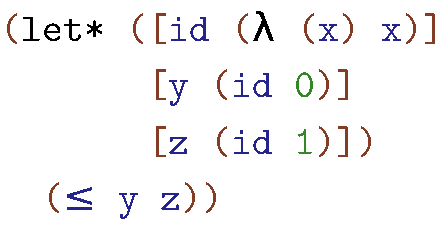
\includegraphics[scale=0.5]{example0}
\end{center}
  % \item{\texttt{(id 0)} steps to \texttt{x} at $\krt{((\texttt{x}, [\texttt{x}\mapsto\texttt{x}]), \mstore_0)}$ with $\mstore_1 =
%     \mstore_0[\texttt{x} \mapsto \set{0}]$ and
%     (let $\mctx_1 = ((\texttt{x},[\texttt{x}\mapsto\texttt{x}]),\mstore_1)$,
%          $\mkont_1 = \klet{\texttt{y}, \texttt{(let ([z (id 1)]) ($\le$ y z))}, [\texttt{id}\mapsto{\texttt{id}}]}$)
%     $\mktab_1 = [\mctx_0 \mapsto \set{\mkont_0}]$}
% \item{\texttt{0} at $\krt{\mctx_1}$ steps to $0$ at $\mkont_1$ and $\mmemo_1 = [\mctx_1 \mapsto \set{0}]$}
% \item{\texttt{0} at $\mkont_1$ steps to \texttt{(let ([z (id 1)]) ($\le$ y z))} and $\mstore_2 = \mstore_1[\texttt{y} \mapsto \set{0}]$}
% \item{\texttt{(let ([z (id 1)]) ($\le$ y z))} steps to \texttt{(id 1)} at \\
%       $\klet{\texttt{z}, \texttt{($\le$ y z)}, [\texttt{id} \mapsto \texttt{id}, \texttt{y} \mapsto \texttt{y}]}$
%       (call this $\mkont_2$).}
% \item{\texttt{(id 1)} steps to $x$ with $\mstore_3 = \mstore_2[\texttt{x} \mapsto \set{0,1}]$ and
%       (let $\mctx_3 = ((\texttt{x},[\texttt{x}\mapsto\texttt{x}]),\mstore_3)$) $\mktab_3 =\mktab_1[\mctx_3 \mapsto \set{\mkont_2}]$.}
% \item{\texttt{0} or \texttt{1} at $\krt{\mctx_3}$ steps to \texttt{0} or \texttt{1} at $\mkont_2$ and $\mmemo_3 = \mmemo_1[\mctx_3 \mapsto \set{0,1}]$.}
% \item{\texttt{z} gets bound to $\set{0,1}$, and \texttt{($\le$ y z)} evaluates to true.}


Suppose we extend our semantics to allow numbers, numeric primitives and \texttt{let}.
%
The continuation frame for a \texttt{let} contains the identifier to bind to the resulting value, along with the body of the \texttt{let} with its environment.
%
Call the constructor of this frame $\mathbf{lt}$.
%%

%%
We should expect that a pushdown analysis would predict this evaluates to true, and there are no loops in the program.
%
0-CFA~\citep{dvanhorn:Shivers:1991:CFA} claims there is a loop from the second call of \texttt{id} to the first, and thus predicts this program evaluates to true or false.
%
PDCFA claims there is no loop and that the result is true.
%
The example evaluation is in \autoref{fig:ex-eval}.
%
Here $\mkont_0 = \mathbf{lt}({\tt y}, {\tt (let\ ([z\ (id\ 1)])\ (}\le\ {\tt y}\ {\tt z))}, \iota)$.
%
We maintain enough context to distinguish the return points of \texttt{id} to not rebind \texttt{y} to 1.
%
When determining control flow through the expression, we consult $\mktab$ to continue past function returns, so there is no confusion about a back edge from the second call to \texttt{id}.
%

\begin{figure}
      % \begin{tabular}{rcccl}
      %   $\begin{array}{l}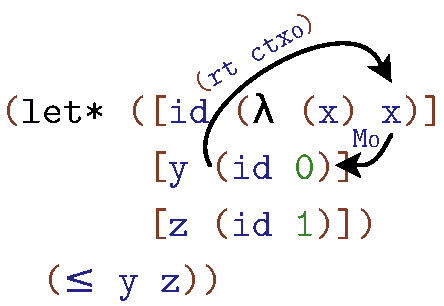
\includegraphics[scale=0.5]{example1}\end{array}$
      %   & $\Rightarrow$ &
      %   $\begin{array}{l}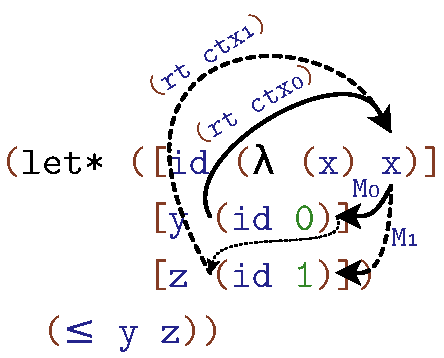
\includegraphics[scale=0.5]{example2}\end{array}$
      %   & $\Rightarrow$ &
      %   $\begin{array}{l}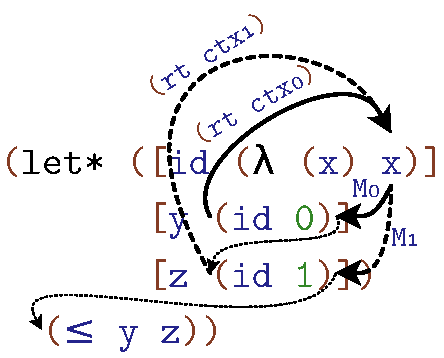
\includegraphics[scale=0.5]{example3}\end{array}$
      % \end{tabular}
      % \begin{center}
      % \begin{tabular}{|l|c|c|c|}
      %   \hline
      %   \# & $\mktab$ & $\mmemo$ \\
      %   \hline
      %   0  & $[\mctx_0 \mapsto \set{\mkont_0}]$ & $[\mctx_0 \mapsto \set{0}]$ \\
      %   1  & $\mktab_0[\mctx_1 \mapsto \set{\mkont_2}]$ & $\mmemo_0[\mctx_1 \mapsto \set{0,1}]$ \\
      %   \hline
      %   \end{tabular}
      % \begin{tabular}{|l|c|}
      %   \hline
      %   \# & $\mctx$ \\
      %   \hline
      %   0  & $(({\tt x}, \iota), \mstore_1)$ \\
      %   1  & $(({\tt x}, \iota), \mstore_3)$ \\
      %   \hline
      % \end{tabular}
      % \begin{tabular}{|l|c|c|}
      %   \hline
      %   \# & $\mstore$ & $\mkont$ \\
      %   \hline
      %   0 & $[{\tt id} \mapsto \set{(\slam{\mvar}{\mvar},\iota)}]$ & $\mkont_0$ \\
      %   1 & $\mstore_0[{\tt \mvar} \mapsto \set{0}]$ & $\krt{\mctx_0}$ \\
      %   2 & $\mstore_1[{\tt y} \mapsto \set{0}]$ & $\mathbf{lt}({\tt z}, {\tt (}\le\ {\tt y}\ {\tt z)}, \iota)$ \\
      %   3 & $\mstore_2[{\tt x} \mapsto \set{0,1}]$ & $\krt{\mctx_1}$ \\
      %   4 & $\mstore_3[{\tt z} \mapsto \set{0,1}]$ & $\kmt$ \\
      %   \hline
      % \end{tabular}
      % \end{center}
\todo{fix example}
      \caption{Example analysis evaluation}
      \label{fig:ex-eval}
\end{figure}
% %% FIXME stores in memo-table
% \begin{enumerate}
% \item{\texttt{(id 0)} steps to \texttt{x} at $\krt{((\texttt{x}, [\texttt{x}\mapsto\texttt{x}]), \mstore_0)}$ with $\mstore_1 =
%     \mstore_0[\texttt{x} \mapsto \set{0}]$ and
%     (let $\mctx_1 = ((\texttt{x},[\texttt{x}\mapsto\texttt{x}]),\mstore_1)$,
%          $\mkont_1 = \klet{\texttt{y}, \texttt{(let ([z (id 1)]) ($\le$ y z))}, [\texttt{id}\mapsto{\texttt{id}}]}$)
%     $\mktab_1 = [\mctx_0 \mapsto \set{\mkont_0}]$}
% \item{\texttt{0} at $\krt{\mctx_1}$ steps to $0$ at $\mkont_1$ and $\mmemo_1 = [\mctx_1 \mapsto \set{0}]$}
% \item{\texttt{0} at $\mkont_1$ steps to \texttt{(let ([z (id 1)]) ($\le$ y z))} and $\mstore_2 = \mstore_1[\texttt{y} \mapsto \set{0}]$}
% \item{\texttt{(let ([z (id 1)]) ($\le$ y z))} steps to \texttt{(id 1)} at \\
%       $\klet{\texttt{z}, \texttt{($\le$ y z)}, [\texttt{id} \mapsto \texttt{id}, \texttt{y} \mapsto \texttt{y}]}$
%       (call this $\mkont_2$).}
% \item{\texttt{(id 1)} steps to $x$ with $\mstore_3 = \mstore_2[\texttt{x} \mapsto \set{0,1}]$ and
%       (let $\mctx_3 = ((\texttt{x},[\texttt{x}\mapsto\texttt{x}]),\mstore_3)$) $\mktab_3 =\mktab_1[\mctx_3 \mapsto \set{\mkont_2}]$.}
% \item{\texttt{0} or \texttt{1} at $\krt{\mctx_3}$ steps to \texttt{0} or \texttt{1} at $\mkont_2$ and $\mmemo_3 = \mmemo_1[\mctx_3 \mapsto \set{0,1}]$.}
% \item{\texttt{z} gets bound to $\set{0,1}$, and \texttt{($\le$ y z)} evaluates to true.}
% \end{enumerate}

\iftr{\subsection{Metatheory}

Correctness follows directly from the invariants we prove of $\mktab$ and $\mmemo$ in the tabular semantics.
%
Allocation strategies are comparable if they produce equal addresses regardless of the differences in the state representations.
%
More formally, $\alloc$ and $\alloc^*$ are comparable if this implication holds:
\begin{mathpar}
  \inferrule{\mkont \in \unroll{\mktab}{\mkont', \emptyset}}
            {\alloc(\tpl{\mpoint,\mstore,\mkont}) = \alloc^*(\tpl{\mpoint,\mstore,\mkont',\mktab,\mmemo})}
\end{mathpar}

The $\mathit{unroll}$ function interprets what are all the valid continuations that $\mktab$ encodes for a given continuation that contains $\krt{\mctx}$, defined as the greatest fixed point of the following rules:
\begin{mathpar}
  \inferrule{ }{\kmt \in \unroll{\mktab}{\kmt, G}} \quad
  \inferrule{\mkont \in \unroll{\mktab}{\mkont', \emptyset}}{\mkframe:\mkont \in \unroll{\mktab}{\mkframe:\mkont', G}} \\
  \inferrule{\mctx \notin G  \\
             \mkont'' \in \mktab(\mctx) \\
             \mkont \in \unroll{\mktab}{\mkont'', \set{\mctx}\cup G}}
            {\mkont \in \unroll{\mktab}{\krt{\mctx}, G}}  
\end{mathpar}

We add $G$ to protect against unguarded corecursion in order for $\mathit{unroll}$ to be well-defined.
%
Interpreting a function with ill-founded recursion can lead to a table such that $\krt{\mctx} \in \mktab(\mctx)$.
%
The abstractions that we impose on our data might also cause this situation, even though the concrete execution might always terminate.

%%
The different tables we have encode information about execution history that we prove is invariant (\autoref{fig:inv}).
%
The first is that the memo table only contains information about previously seen contexts; we need this to infer that there was at least one call leading to the memoized context such that we can use stack irrelevance to justify skipping to the memoized result.
%
The second, $\phi_{\reachable}$, states that all the calling contexts in the continuation table reach some unrolling of the current state.
%
The final invariant, $\phi_{\memo}$, states that all paths starting at a function call either reach the memoized result, or if the path does not include a return, there is an extension that will.
%
The portion of these paths between call and return hal the calling context's continuation in the tail to justify using stack-irrelevance.

\begin{figure}
  \centering
  \begin{align*}
    \inv(\tpl{\mpoint, \mstore, \mkont, \mktab, \mmemo}) &=
    \dom(\mmemo) \subseteq \dom(\mktab) \\
    &\wedge \forall (\mpoint',\mstore') \in \dom(\mktab), \mkont''
    \in \mktab(\mpoint',\mstore'),
    \mkont' \in \unroll{\mktab}{\mkont'', \emptyset}. \\
    &\qquad \phi_{\reachable} \wedge \phi_{\memo} \\
    \text{where } \phi_{\reachable} &= \exists \mkont'' \in
    \unroll{\mktab}{\mkont,\emptyset}.
    \tpl{\mpoint', \mstore', \mkont'} \stepto^* \tpl{\mpoint, \mstore, \mkont''} \\
    \phi_{\memo} &=
    \forall (\mval, \mstore'') \in \mmemo(\mpoint',\mstore'). \\
    &\qquad\exists \mtrace\equiv\tpl{\mpoint', \mstore', \mkont'} \stepto^* \tpl{\mval,\mstore'',\mkont'}. \hastail(\mtrace,\mkont')
  \end{align*}
  \caption{Table invariants}
\label{fig:inv}
\end{figure}
\begin{lemma}[Table invariants in CESK$\mathit{\Xi{}M}$]\label{lem:tab-inv}
  If $\inv(\mstate)$ and $\mstate \stepto \mstate'$ then $\inv(\mstate')$.
\end{lemma}
\begin{proof}
  By cases on $\stepto$.
  \begin{byCases}
% variable lookup
    \case{\tpl{(\svar\mvar, \menv), \mstore, \mkont, \mktab, \mmemo}
          \stepto
          \tpl{\mval,\mstore,\mkont, \mktab, \mmemo} \text{ if }\mval \in \mstore(\menv(\mvar))}{
     Same continuation and tables, so holds by $\inv(\mstate)$.}
% application
    \case{\tpl{(\sapp{\mexpri0}{\mexpri1}, \menv), \mstore, \mkont, \mktab, \mmemo}
          \stepto
          \tpl{(\mexpri0, \menv), \mstore, \kcons{\kar{\mexpri1,\menv}}{\mkont}, \mktab, \mmemo}}{
    Let $\mctx, \mkont^\circ, \mkont'$ be arbitrary.
    Let $\mkont^*$ be the witness for $\mstate$.
    The next witness is $\kcons{\kar{\mexpri1,\menv}}{\mkont^*}$, by definition of $\mathit{unroll}$.}
% argument evaluation
    \case{\tpl{\mval, \mstore, \kcons{\kar{\mexpr,\menv}}{\mkont}, \mktab, \mmemo}
          \stepto
          \tpl{(\mexpr, \menv), \mstore, \kcons{\kfn{\mval}}{\mkont}, \mktab, \mmemo}}{
    Let $\mctx, \mkont^\circ, \mkont'$ be arbitrary.
    Let $\kcons{\kar{\mexpr,\menv}}{\mkont^*}$ be the witness for $\mstate$.
    The next witness is $\kcons{\kfn{\mval}}{\mkont^*}$, by definition of $\mathit{unroll}$.}
% function call
    \case{\tpl{\mval,\mstore,\kcons{\kfn{\vclo{\slam{\mvar}{\mexpr}}{\menv}}}{\mkont},\mktab,\mmemo}
          \stepto
          \tpl{\mpoint, \mstore', \krt{\mpoint, \mstore'}, \mktab', \mmemo}}{
     where
     $\begin{array}{l}
       \mpoint = (\mexpr, \extm{\menv}{\mvar}{\maddr}) \\
       \mstore' = \joinone{\mstore}{\maddr}{\mval} \\
       \mktab' = \joinone{\mktab}{(\mpoint, \mstore')}{\mkont}
     \end{array}$ \\

    Let $\mctx, \mkont^\circ, \mkont'$ be arbitrary.
    Let $\kcons{\kfn{\mval}}{\mkont^*}$ be the witness for $\mstate$.
    The next witness is $\mkont^*$, by definition of $\mathit{unroll}$.}
% memo-lookup
    \case{\tpl{\mval,\mstore,\kcons{\kfn{\vclo{\slam{\mvar}{\mexpr}}{\menv}}}{\mkont},\mktab,\mmemo}
          \stepto
          \tpl{\mval_\mathit{result}, \mstore'', \mkont, \mktab', \mmemo}
          \text{ if } (\mval_\mathit{result},\mstore'') \in \mmemo(\mpoint,\mstore')}{
        same where clause as previous case.
     
    Let $\mctx, \mkont^\circ, \mkont'$ be arbitrary.
    By definition of $\inv$, and since $\tpl{\mpoint',\mstore',\mkont'} \stepto^* \tpl{\mval_{\mathit{result}}, \mstore'', \mkont'}$.
    For the memo entry to exist, there must have been at least one previous continuation in $\mktab(\mpoint',\mstore')$.
    We use $\inv$ with this continuation, combined with stack irrelevance to produce the trace involving $\mkont'$.
    }
% return
    \case{\tpl{\mval, \mstore, \krt{\mpoint,\mstore'}, \mktab, \mmemo}
          \stepto
          \tpl{\mval, \mstore, \mkont, \mktab, \joinone{\mmemo}{(\mpoint, \mstore')}{(\mval,\mstore)}}
          \text{ if } \mkont \in \mktab(\mpoint, \mstore')}{
    Let $\mctx, \mkont^\circ, \mkont'$ be arbitrary.
    $\mkont'$ is an acceptable witness for the first property.
    The path we construct to $\mstate'$ is sufficient for the second property.}
  \end{byCases}
\end{proof}

In order to prove this, we need a lemma that allows us to plug in any continuation for memoized results.
%
When traces (sequences of states such that adjacent states are related by $\stepto$) have a common tail, we can replace it with anything.

\begin{lemma}[Stack irrelevance in CESK]\label{lem:irrelevance}
  $\hastail(\mtrace,\mkont)$ implies $\replacetail(\mtrace,\mkont,\mkont')$ is a valid trace.
\end{lemma}
\begin{proof}
  By induction on $\mtrace$. Base cases trivially hold, and induction step follows from cases on $\mstate \stepto \mstate'$ and definition of $\replacetail$.
\end{proof}

\begin{mathpar}
  \inferrule{ }{\hastail(\epsilon,\mkont)} \quad
  \inferrule{ }{\hastail(\tpl{\mpoint,\mstore,\append{\mkont'}{\mkont}},\mkont)} \quad
  \inferrule{\hastail(\mtrace\mstate,\mkont) \quad
             \mstate \stepto \mstate' \quad
             \hastail(\mstate',\mkont)}
            {\hastail(\mtrace\mstate\mstate',\mkont)}
\end{mathpar}

\begin{align*}
  \replacetail(\tpl{\mpoint,\mstore,\append{\mkont'}{\mkont}},\mkont,\mkont'') &= \tpl{\mpoint,\mstore,\append{\mkont'}{\mkont''}} \\
  \replacetail(\epsilon,\mkont,\mkont'') &= \epsilon \\
  \replacetail(\mtrace\mstate,\mkont,\mkont') &= \replacetail(\mtrace,\mkont,\mkont')\replacetail(\mstate,\mkont,\mkont') \\
\end{align*}

\begin{theorem}[Correctness of Concrete Summarization]\label{thm:concrete-tabular}
  The standard semantics has a skipping bisimulation with the tabular semantics given comparable fresh allocation strategies.
\end{theorem}
\begin{proof}[Sketch]
  The tabular semantics skipping simulates that standard semantics by appealing to the table invariants to show the long ``recomputation'' path.
  Crucially, since the memo table is only set once before being used to bypass to the result, there must be only one possible result in the standard semantics. Otherwise, the tabular semantics would miss out on the other results for subsequent calls with the same context.
  The fresh allocation strategy ensures that relation is deterministic and thus function calls only reduce to one result.

  The standard semantics skipping simulates the tabular semantics because ``recomputing'' paths always have the calling stack as its tail, so we can step forward on the invariant's inductively built path until the result.
\end{proof}

Finally, we can show that the reductions we find between states paired with the shared tables define a sound and complete abstraction of the CESK machine with a comparable allocation strategy.
}

\section{Deriving GC from the introspective pushdown model}\label{sec:gc}

Abstract garbage collection~\citep{dvanhorn:Might:2006:GammaCFA} is a powerful technique for regaining precision in an abstract interpretation.
%
The followup to PDCFA~\citep{dvanhorn:Earl2012Introspective} that allows inspecting the stack in order to perform sound GC introduces an entirely new class of automata for this one purpose.
%
In our view with tabular semantics, the GC story mimics the simplicity of GC in the regular setting, without the detour into automata theory.
%
We follow the GC style of \citet{dvanhorn:Might:2006:GammaCFA} with a stop-and-copy collector.
%
Address reachability is in terms of a base ``touches'' function, $\touches$.
%
Entries in $\mktab$ might be circular, so we compute the continuation frames in a fixed-point before computing touched addresses:
\begin{center}
  \,
    $\touchesk{\mkont}(\mktab) = \setbuild{\maddr}{\mkont \rightsquigarrow_\mktab^*\maddr}$
\\[4pt]
  \begin{minipage}{0.55\linewidth}
    $\touchesf(\kar{\mexpr,\menv}) = \mathit{range}(\menv|_{\mathit{fv}(\mexpr)})$
  \end{minipage}
  \begin{minipage}{0.4\linewidth}
    $\touchesf(\kfn{\mval}) = \touches(\mval)$
  \end{minipage}
\end{center}
\begin{mathpar}
  \inferrule{ }{\kcons{\mkframe}{\mkont} \rightsquigarrow_\mktab \mkont}
  \quad
  \inferrule{\maddr \in \touchesf(\mkframe)}{\kcons{\mkframe}{\mkont} \rightsquigarrow_\mktab \maddr}
  \quad
  \inferrule{\mkont \rightsquigarrow_\mktab \mkont'}{\kcons{\mkframe}{\mkont} \rightsquigarrow_\mktab \mkont'}
  \quad
  \inferrule{\mkont \rightsquigarrow_\mktab \maddr}{\kcons{\mkframe}{\mkont} \rightsquigarrow_\mktab \maddr}
%  \inferrule{\mkont \rightsquigarrow_\mktab (\mkont' \text{ or } \maddr)}{\kcons{\mkframe}{\mkont} \rightsquigarrow_\mktab (\mkont' \text{ or } \maddr)}
  \\
  \inferrule{\mkont \in \mktab(\mctx)}{\krt{\mctx} \rightsquigarrow_\mktab \mkont}
\end{mathpar}

Garbage collection ($\Gamma$) restricts the heap to just the reachable addresses, so a semantics with GC introduces the following reduction rule:
\begin{center}
  \begin{minipage}{0.3\linewidth}
    \begin{align*}
      \mstate \stepto \Gamma(\mstate)
    \end{align*}
  \end{minipage}
  \begin{minipage}{0.65\linewidth}
    \begin{align*}
      \Gamma(\tpl{\mexpr,\menv,\mstore,\mkont, \mktab, \mmemo}) &= \tpl{\mexpr,\menv,\mstore|_{\reaches(\mathit{root}, \mstore)}, \mkont, \mktab, \mmemo} \\
      \text{where } \mathit{root} &= \touchesk{\mkont}(\mktab) \cup
      \mathit{range}(\menv|_{\mathit{fv}(\mexpr)})
    \end{align*}
  \end{minipage}
\end{center}
%
The ``reaches'' metafunction ($\reaches$) is a transitive closure of ``touches'' as it weaves through the store, starting from some root set of addresses:

\begin{center}
  $\reaches(\mathit{root}, \mstore) = \setbuild{b}{\maddr \in \mathit{root}, \maddr \rightsquigarrow_\mstore^* b}$
\end{center}
\begin{mathpar}
  \inferrule{\mval \in \mstore(\maddr) \\
    b \in \touches(\mval)}
  {\maddr \rightsquigarrow_\mstore b}
\end{mathpar}

This semantics of course enjoys the soundness properties that GC does not introduce dangling pointers, equal length traces are equal up to GC (in the concrete), and abstractions are sound with respect to collected states.
%
The proofs are all similar to the original abstract GC paper's.
%
Technically since this semantics inspects the touched addresses of the continuation, the set of touched addresses should be considered part of the ``context'' in the $\mathbf{rt}$ continuations.
%
This extra context can be overlooked, but it leads to larger live address sets.
%
More live addresses means a less effective GC, but the introspective pushdown analysis chose this tradeoff for a possibly smaller state space.
%

\section{Deriving CFA2}
\label{sec:cfa2}

The creators of CFA2 had a clear goal of harnessing the extra information a pushdown model provides to produce a high-precision analysis that works well in practice.
%
This resulted in the following features in addition to just the call/return matching of \autoref{sec:pdcfa}:
%

\begin{enumerate}
\item{stack allocation for some bindings in an additional $\mframe \in \Store$}
\item{strong updates on stack frames for looked-up addresses}
\end{enumerate}
There are two orthogonal features of the semantics, embodied by our semantics' two metafunctions ($\bind$ and $\lookup$, respectively in \autoref{fig:frame-semantics}).

\begin{figure}
  \centering
  $\mstate \stepto \mstate' \text{ where } \maddr = \alloc(\mstate)$ \\
  \begin{tabular}{r|l}
    \hline
% variable lookup
    $\tpl{\svar[\mlab]{\mvar}, \menv, \mstore, \mframe, \mkont}$
    &
    $\tpl{\mval,\mstore,\mframe',\mkont}$
    \\ & if $(\mframe', \mval) \in \lookup(\mstore,\mframe,\menv(\mvar),\mlab)$
    \\
% % application
%     $\tpl{(\sapp{\mexpri0}{\mexpri1}, \menv), \mstore, \mframe, \mkont}$
%     &
%     $\tpl{(\mexpri0, \menv), \mstore, \mframe, \kar{\mexpri1,\menv,\mkont}}$
%     \\
% % argument evaluation
%     $\tpl{\mval, \mstore, \mframe, \kar{\mexpr,\menv,\mkont}}$
%     &
%     $\tpl{(\mexpr, \menv), \mstore, \mframe, \kfn{\mval, \mkont}}$
%     \\
% function call
    $\tpl{\mval,\mstore,\mframe,\kcons{\kfn{\vclo{\slam{\mvar}{\mexpr}}{\menv}}}{\mkont}}$
    &
    $\tpl{\mexpr, \extm{\menv}{\mvar}{\maddr}, \mstore', \mframe', \kcons{\kpush{\mframe}}{\mkont}}$
    \\ & where $(\mstore',\mframe') = \bind(\mstore,\maddr,\mvar,\mval)$
    \\
    $\tpl{\mval,\mstore,\mframe,\kcons{\kpush{\mframe'}}{\mkont}}$
    &
    $\tpl{\mval,\mstore,\mframe',\mkont}$
  \end{tabular}
  \caption{The CES$\xi$K machine significant rules}
  \label{fig:frame-semantics}
\end{figure}

%
There is a conservative pre-analysis that checks locally whether a binding will never escape, and classifies references (labeled with a distinguishing $\mlab$ from an arbitrary space of labels) as able to use the stack frame or not.
%
We will call the non-escaping conditions ``local.''
%
%Their criteria for a binding never escaping is like the criteria of register-allocatable bindings in the Orbit Scheme compiler~\citep{ianjohnson:kranz:thesis:1988}.
%
CFA2 uses the information that a binding never escapes to not bother allocating it in the heap.
%
This has the advantage of not changing the heap, and thus leads to less propagation.
%
The addition of these stack frames makes the analysis exponential in theory, though in practice they have been observed to decrease running time in most cases.
%%

%%
The second of these is to ameliorate a problem they call ``fake rebinding.''
%
Bindings in the abstract represent several values, but we don't want to reference a variable \texttt{x} in different places in a function and have it resolve to different values
\footnote{In AAM, a variable reference non-deterministically steps to all possible values associated with that variable.}.
%
If subsequent variable references are not the same, it looks as if the variable was rebound; it hasn't, and thus it is a ``fake rebinding.''
%
Model-checking literature has \emph{explicit} constructs to locally bind the result of this non-deterministic choice: \emph{choice variables}~\citep{ianjohnson:DBLP:conf/spin/CookKS05, ianjohnson:DBLP:journals/cacm/DilligDA10}.
%
%CFA2 does not step to all values on variable reference, but instead carries all its values around in superposition until they need to be observed at, say, a function call.
%
%We give a simplified semantics that is more along the AAM style, but CFA2's approach can easily be recovered from it.\footnote{Our Redex model implements the fake rebinding strategy CFA2 itself employs.}
%%

%%
CFA2 uses a ``local semantics'' that is similar to our segmenting continuations at function boundaries, but gets stuck when it gets to a point where it would need to ``return.''
%
Returns are un-stuck by an imperative summarization algorithm driving the state exploration.
%
What we show here is almost wholly the same in character, only embodied still in terms of a machine semantics and thus more easily reasoned about, and can be run in the concrete.
%%

%%
We show only the significantly modified rules of the semantics in \autoref{fig:frame-semantics}.
%
%The other rules simply carry along the extra $\mframe$ component untouched.
%
The meta-functions the semantics uses to extend and consult the heap and stack use implicit information from the pre-analysis we described above:

\begin{align*}
  \bind(\mstore,\maddr,\mvar,\mval) &=
   \left\{\begin{array}{ll}
            (\mstore, \snglm{\maddr}{\mval}) &\text{ if } \mvar \text{ local} \\ % allocations never escape
            (\joinone{\mstore}{\maddr}{\mval}, \snglm{\maddr}{\mval}) &\text{ otherwise} \\
          \end{array}\right. \\
  \lookup(\mstore,\mframe,\maddr,\mlab) &=
    \left\{\begin{array}{ll}
          \setbuild{(\extm{\mframe}{\maddr}{\set{\mval}}, \mval)}
                   {\mval \in \mframe(\maddr)} & \text{if } \mlab \text{ local} \\ %non-escaping
          \setbuild{(\mframe,\mval)}{\mval \in \mstore(\maddr)} & \text{ otherwise}
           \end{array}\right.
\end{align*}

Sidestepping fake rebinding does not need to be restricted to stackable references, but that is what CFA2 does.
%
As soon as the non-determinism has been determined, we could extend the stack frame so any subsequent reference means what it meant previously in the function.
%
Look-up would then always try the stack frame before falling back on the heap, though this must be limited to immutable addresses.
%%

A tabular semantics for the CES$\xi$K machine follows the previous section, except that $\mktab$ now stores $(\mkont, \mframe)$ pairs, and returns reinstate the saved $\mframe$:
\begin{align*}
  \tpl{\mval,\mstore,\mframe,\kcons{\kfn{\slam{\mvar}{\mexpr},\menv}}{\mkont},\mktab,\mmemo} &\stepto
  \tpl{\mpoint,
    \mstore',
    \mframe',
    \krt{\mpoint, \mstore'},
    \mktab',
    \mmemo} \\
  \text{where }
  & \mpoint = (\mexpr, \extm{\menv}{\mvar}{\maddr}) \\
  & (\mstore',\mframe') = \bind(\mstore,\maddr,\mvar,\mval) \\
  & \mktab' = \joinone{\mktab}{(\mpoint, \mstore')}{(\mkont,\mframe)}
\\[2pt]
 \tpl{\mval, \mstore, \mframe, \krt{\mpoint,\mstore'}, \mktab, \mmemo} &\stepto
 \tpl{\mval, \mstore, \mframe', \mkont, \mktab, \mmemo'}
  \\ & \quad\text{if } (\mkont,\mframe') \in \mktab(\mpoint, \mstore')
  \\ \text{where } & \mmemo' = \joinone{\mmemo}{(\mpoint, \mstore')}{(\mval,\mstore)}
\end{align*}

%%
%% CFA2 also includes what they called ``transitive summaries'' to deal with tail calls.
%% %
%% We create an $\rt$ continuation at every function call.
%% %
%% This view contends with tail calls, but we can identify tail calls easily---any call with an $\rt$ as its continuation is a tail call.
%% %
%% Tail calls are important in language implementations for space complexity reasons \citep{ianjohnson:clinger:tail-calls:1998}, but in an analysis, these concerns are less important since there is no unbounded recursion.
%% %
%% The repeated popping of $\rt$ inserted by what otherwise were tail-calls is synonymous with CFA2's transitive summaries.

\paragraph{Example:} revising the earlier example, we find that with the addition of stack frames, there is no confusion about \texttt{z}'s value either.
%
If the operator were instead $<$ or $+$, we could still constant fold that away.
%%

%%
The stack frame introduces a refinement over the original CESK machine, so we first prove it correct with respect to the concrete semantics, in a similar fashion to PDCFA.
%
\begin{theorem}[Correctness of stack frame refinement]\label{thm:refinement}
  The CES$\xi$K machine has a stuttering bisimulation refinement with the CESK machine with fresh allocation.
\end{theorem}
This follows from the invariant that if a stack frame maps $\maddr$ to $\mval$, then the store maps $\maddr$ to $\mval$, meaning that the special lookup function is equivalent to lookup directly in the store (exploits immutability).
%
We stutter past the stack frame replacement steps.
%
%That is, if we always allocated bindings in the heap.
%
%The additional escape information that allows us to elide allocation in the heap introduces a second level of reasoning, where the burden of proof falls on the escape analysis.
%
%The escape analysis adds information to use in the proof, that if $\mvar$ never escapes, then every reference to allocations of $\mvar$'s binding will always be able to use $\mframe$ for the lookup.
%
%With this proposition, we can prove that the CES$\xi$K machine that always allocates in the store has a bisimulation with the refined machine that exploits escape analysis to avoid unnecessary changes to the store.
%

\begin{theorem}[Correctness of CFA2]\label{thm:cfa2}
  The widened tabular semantics reflects a relation that has a bisimulation with the CES$\xi$K machine.
\end{theorem}
%This proof has the same structure as that of PDCFA.

\ifwcm{
\section{Stack inspection with continuation marks}
\label{sec:wcm}

We saw in \autoref{sec:gc} that a semantics can inspect the continuation table to compute a property of the ``whole stack,'' which is outside the model of pushdown systems.
%
Here we show that Clements and Felleisen's WCM machine (a generalization of the CM machine) is directly analyzable in this setting, though we give up some precision in order to account for all calling contexts instead of the single one a function is currently in.
%
The machine can extend the marks of the continuation, reify the current set of marks, and query the set for all the values given to a particular mark key.
%
The mark set of the continuation is then part of the ``context'' for function calls, since functions can inspect the marks.
%
Mark sets can have unbounded length chains of values for each mark key, so we use $\alloc$ to tune the precision of context comparisons.
%
The effect is that we reify the current mark set for each function call to keep as part of the context (one can devise caching strategies for better performance).
%
We use a private store to represent the chains of values, in order to not affect the precision of reifications that happen within the analyzed program.
%
\begin{align*}
  \mexpr \in \Expr &::= \swcm{\mexpr}{\mexpr}{\mexpr} \alt \sccms \alt \scmsl{\mexpr}{\mexpr} \alt \ldots \\
  \mctx \in \Context &::= (\mexpr, \menv, \mstore, \mmarkset) \\
  \mkframe \in \Frame &::= \kwcmk{\mexpr, \mexpr, \menv} \alt
                           \kwcmv{\mval, \mexpr, \menv} \alt
                           \kcmsls{\mexpr,\menv} \alt
                           \kcmslk{\mval} \alt \kwcm{\mmarks} \alt \ldots \\
  \mkont \in \Kont &::= \kmt^\bot \alt \krt{\mctx}^\mmarks \alt \kcons{\mkframe^\mmarks}{\mkont} \\
  \mmarks \in \Marks &= \Value \to \wp(\Value) \\
  \mmarkset \in \Markset &= \Marks \times \Store \\
  \mval \in \Value &::= \texttt{nil} \alt \cons{\maddr}{\maddr} \alt \smarkset{\mmarks} \alt \ldots
\end{align*}

%% TODO: distinguish between copied and extended marks so that domarkset only builds
%% a list of mark extensions
\begin{figure}
  \centering
  $\mstate \stepto \mstate' \text{ where } \maddr = \alloc(\mstate)$ \\
  \begin{tabular}{r|l}
    \hline
% wcm eval key
    $\tpl{\swcm{\mexpr_k}{\mexpr_v}{\mexpr}, \menv, \mstore, \mkont^\mmarks, \mktab, \mmemo}$
    &
    $\tpl{\mexpr_k, \menv, \mstore, \kcons{\kwcmk{\mexpr_v,\mexpr,\menv}^\mmarks}{\mkont}, \mktab, \mmemo}$
    \\
% wcm eval value
    $\tpl{\mval_k, \mstore, \kcons{\kwcmk{\mexpr_v,\mexpr,\menv}}{\mkont^\mmarks}, \mktab, \mmemo}$
    &
    $\tpl{\mexpr_v, \menv, \mstore, \kcons{\kwcmv{\mval_k,\mexpr,\menv}^\mmarks}{\mkont}, \mktab, \mmemo}$
    \\    
% wcm all done.
    $\tpl{\mval_v, \mstore, \kcons{\kwcmv{\mval_k, \mexpr, \menv}}{\mkont}, \mktab, \mmemo}$
    &
    $\tpl{\mexpr,\menv,\mstore,\mkont',\mktab', \mmemo}$ \\
    where & $(\mkont',\mktab') = \domark(\mkont,\mktab,\mval_k,\mval_v)$
    \\
% Pop marks
   $\tpl{\mval,\mstore,\kcons{\kwcm{\mmarks}^{\mmarks'}}{\mkont}, \mktab, \mmemo}$
   &
   $\tpl{\mval,\mstore,\mkont,\mktab,\mmemo}$
   \\
% function call
    $\tpl{\mval,\mstore,\kcons{\kfn{\vclo{\slam{\mvar}{\mexpr}}{\menv}}^\mmarks}{\mkont}}$
    &
    $\tpl{\mexpr, \menv', \mstore', \krt{\mctx}^\mmarks,\mktab',\mmemo}$
    \\ where & $\menv' = \extm{\menv}{\mvar}{\maddr}$ \\
    & $\mstore' = \joinone{\mstore}{\maddr}{\mval}$ \\
    & $\mctx = (\mexpr,\menv',\mstore', \domarkset(\mstate))$ \\
    & $\mktab' = \joinone{\mktab}{\mctx}{\mkont}$
    \\
% Current continuation marks
    $\tpl{\sccms,\menv,\mstore,\mkont,\mktab,\mmemo}$
    &
    $\tpl{\smarkset{\mmarks},\mstore\sqcup\mstore',\mkont,\mktab,\mmemo}$
    \\ where & $(\mmarks,\mstore') = \domarkset(\mstate)$
    \\
% cms->list mark set
    $\tpl{\scmsl{\mexpr_\mmarks}{\mexpr_k}, \menv, \mstore, \mkont^\mmarks, \mktab, \mmemo}$
    &
    $\tpl{\mexpr_\mmarks, \menv, \mstore, \kcons{\kcmsls{\mexpr_k,\menv}^\mmarks}{\mkont}, \mktab, \mmemo}$
    \\
% cms->list key
    $\tpl{\mval, \mstore, \kcons{\kcmsls{\mexpr_k,\menv}}{\mkont^\mmarks}, \mktab, \mmemo}$
    &
    $\tpl{\mexpr_k, \menv, \mstore, \kcons{\kcmslk{\mval}^\mmarks}{\mkont}, \mktab, \mmemo}$
    \\
% cms->list done
    $\tpl{\mval_k, \mstore, \kcons{\kcmslk{\mmarks}}{\mkont}, \mktab, \mmemo}$
    &
    $\tpl{\mval, \mstore, \mktab, \mmemo}$ if $\mval \in \mmarks(\mval_k)$
  \end{tabular}  
  \caption{The Tabular WCM machine (list rules not shown)}
  \label{fig:wcm}
\end{figure}

The two metafunctions, $\domark$ and $\domarkset$ are what do the heavy-lifting of adding marks to a continuation and reifying the mark set into a map of keys to lists.
%
Adding a mark to a continuation has an implicit equality check; if $\mval_k = \mval_k'$ concretely, then {\tt wcm} should do a strong update on $\mmarks$, but otherwise it should join since they could be two different values.
%
Concrete equality analysis is outside the scope of this paper, but doable (\eg, with abstract counting~\citep{dvanhorn:Might:2006:GammaCFA}), so we elide the details and call this strong-update-or-join operation $\sqcup_{!{}}$.
%
Marking a return continuation means we need to crawl through the table, which again can be circular, so we compute the least fixed point of ${\mathcal M}$ to get an extended table holding the marked continuations.
%
\newcommand{\rewritectx}{\mathit{rw}}
\newcommand{\domarkstep}{\mathit{mark}_0}
\begin{align*}
  \domark(\mkont, \mktab, \mval_k, \mval_v) &= (\mkont', \mktab) \text{ if } (\mkont',\bot) = \domarkstep(\mkont) \\
  \domark(\mkont, \mktab, \mval_k, \mval_v) &= (\mkont', \mathbf{snd}(\lfp({\mathcal M}(\mctx)))) \text{ if } (\mkont',\mctx) = \domarkstep(\mkont) \\
  \text{where } {\mathcal M}(\mctx_0)(C, \mktab) &= (C \cup C' \cup \set{\mctx_0}, \mktab \sqcup \mktab') \\
    I &= \setbuild{(\rewritectx(\mctx), \setbuild{\domarkstep(\mkont')}{\mkont' \in \mktab(\mctx)})}{\mctx \in C} \\
    C' &= \setbuild{\mctx}{(\_, S) \in I, (\_, \mctx) \in S} \\
    \mktab' &= \bigsqcup\setbuild{[\mctx \mapsto \setbuild{\mkont}{(\mctx, S) \in I, (\mkont, \_) \in S}]}{(\mctx,\_) \in I}
\\[2pt]
  \rewritectx(\mexpr,\menv,\mstore,(\mmarks, \mstore')) &= (\mexpr,\menv,\mstore,(\mmarks\sqcup_{!{}}[\mval_k \mapsto \mval_v], \mstore'))
\\[2pt]
  \domarkstep(\krt{\mctx}^\mmarks) &= (\krt{\rewritectx(\mctx)}^{\mmarks \sqcup_{!{}} [\mval_k \mapsto \mval_v]}, \mctx) \\
  \domarkstep(\kcons{\kwcm{\mmarks}^{\mmarks'}}{\mkont}) &= (\kcons{\kwcm{\mmarks \sqcup_{!{}} [\mval_k \mapsto \mval_v]}^{\mmarks' \sqcup_{!{}} [\mval_k \mapsto \mval_v]}}{\mkont}, \bot) \\
  \domarkstep(\mkont^\mmarks) &= (\kcons{\kwcm{[\mval_k \mapsto \mval_v]}^{\mmarks \sqcup_{!{}} [\mval_k \mapsto \mval_v]}}{\mkont}, \bot)
\end{align*}

Second, the $\domarkset$ metafunction builds a map of keys to lists, and builds a private store for the list constructions.
%
For this, we extend $\alloc$'s specification to allow more arguments---the private store, and a set of keys that need cons cells allocated for them---and produce a map from keys to pairs of addresses.
%
%% FIXME: need to crawl through qualified continuations for all extensions to build a list for each found key.
%% Has another implicit equality check
\newcommand{\markaux}{\mathit{marks}}
\begin{align*}
  \domarkset(\mstate\equiv\tpl{\mpoint,\mstore,\mkont,\mktab,\mmemo}) &= \markaux(\mkont,\emptyset) \\
  \markaux(\kmt^\bot, G) &= (\bot, \bot) \\
  \markaux(\krt{\mctx}^\mmarks, G) &= (\bot, \bot) \text{ if } \mctx \in G \\ %% FIXME: unsound
  \markaux(\krt{\mctx}^\mmarks, G) &= \bigsqcup\limits_{\mkont\in \mktab(\mctx)}{\markaux(\mkont,G \cup \set{\mctx})} \text{ otherwise} \\
  \markaux(\kcons{\kwcm{\mmarks}^{\mmarks'}}{\mkont}, G) &= (\mmarks''[\mval_k \mapsto \set{\cons{a}{d}} : \mval_k \in \dom(\mmarks), (a, d) = A(\mval_k)], \\
    &\phantom{= (}
      \mstore\sqcup[a \mapsto \mmarks(\mval_k) : \mval_k \in \dom(\mmarks), (a,\_) = A(\mval_k)] \\
    &\phantom{= (\mstore}\sqcup[d \mapsto \mmarks''(\mval_k) : \mval_k \in \dom(\mmarks), (\_,d) = A(\mval_k)]
   \\ \text{where } (\mmarks'', \mstore) &= \markaux(\mkont, G)
   \\ A &= \alloc(\mstate, \mstore, \dom(\mmarks))
\end{align*}
}

\section{Analysis of delimited, composable control}
\label{sec:sr}

%% (thanks to ccshan): Discuss difference between CPS for shift/reset and this approach,
%% Discuss how this does not generalize to first class prompts due to append versus cons.

%% TODO: Cut here next.
There is contention among programming language researchers whether \rackett{call/cc} should be a language primitive\citep{ianjohnson:kiselyov:against-callcc}.
%
Alternative control operators have been proposed that delimit how much of the stack to capture, such as $\%$ (read ``prompt'') and capture operator ${\mathcal F}$ (read ``control'') \citep{ianjohnson:felleisen:control:1988}, or \texttt{reset} and \texttt{shift} \citep{ianjohnson:danvy:filinski:delim:1990}.
%
However, the stacks captured by these operators always extend the stack when invoked, rather than replace it like those captured with \rackett{call/cc}.
%
Continuations that have this extension behavior are called ``composable continuations.''
%
Stack extension poses a new challenge for pushdown analysis, since one application of a composable continuation means pushing an unbounded amount of frames onto the stack.
%
Vardoulakis' and Shivers' technique drops all knowledge of the stack at a continuation's invocation site; extension must preserve it.
%%

%%
The way we have been splitting continuations at function calls has similarities to the meta-continuation approach to modeling delimited control, given in figure \ref{fig:shift-reset} (adapted from~\citep{ianjohnson:Biernacki2006274}).
%
We could view each function call as inserting a prompt, and returns as aborting to the nearest prompt.
%
Resets then insert a second-tier prompt.
%
The changed semantic spaces for the shift/reset semantics are as follows:

\begin{center}
  \begin{minipage}{0.45\linewidth}
    \begin{align*}
      \mstate \in \State &::= \tpl{\mpoint, \mstore, \mkont, \mmkont} \\
      \mpoint \in \Point &::= (\mexpr, \menv) \alt \mval
    \end{align*}
  \end{minipage}
  \begin{minipage}{0.50\linewidth}
    \begin{align*}
      \mval \in \Value &::= \vclo{\slam{\mvar}{\mexpr}}{\menv} \alt \vcomp{\mkont} \\
      \mmkont \in \MKont &::= \kmt \alt \mkapp{\mkont}{\mmkont}
    \end{align*}
  \end{minipage}
\end{center}
\begin{figure}
  \centering
  $\mstate \stepto \mstate' \text{ where } \maddr = \alloc(\mstate)$ \\
  \begin{tabular}{r|l}%{r|ll}
    \hline
% Reset
    $\tpl{\sreset{\mexpr}, \menv, \mstore, \mkont, \mmkont}$
    &
    $\tpl{\mexpr, \menv, \mstore, \kmt, \mkapp{\mkont}{\mmkont}}$
%    & \textsc{[push prompt]}
    \\
% Pop prompt
    $\tpl{\mval, \mstore, \kmt, \mkapp{\mkont}{\mmkont}}$
    &
    $\tpl{\mval, \mstore, {\mkont}, {\mmkont}}$
%    & \textsc{[pop prompt]}
    \\
% Shift
    $\tpl{\sshift{\mvar}{\mexpr}, \menv, \mstore, \mkont, \mmkont}$
    &
    $\tpl{\mexpr, \extm{\menv}{\mvar}{\maddr}, \mstore',\kmt,\mmkont}$
%    & \textsc{[capture continuation]}
    \\ where & $\mstore' = \joinone{\mstore}{\maddr}{\vcomp{\mkont}}$
    \\
% continuation call
    $\tpl{\mval,\mstore,\kcons{\kfn{\vcomp{\mkont'}}}{\mkont}, \mmkont}$
    &
    $\tpl{\mval, \mstore, \mkont', \mkapp{\mkont}{\mmkont}}$
%    & \textsc{[compose continuation]}
  \end{tabular}  
  \caption{Machine semantics for shift/reset}
  \label{fig:shift-reset}
\end{figure}

The table-based semantics makes prompts a point of indirection, just like function calls.
%
Memoization also gets a new context to consider, calling a continuation, because composable continuations act like functions.
%
We separate contexts stored in meta-continuations from those in continuations to avoid losing precision from abstracting continuations' contexts.
%
The table for continuations is treated the same way as in the previous semantics for standard function call and return.
%
The new semantic spaces are then

\begin{align*}
  \mctx \in \Context &::= (\mexpr,\menv,\mstore) \alt (\vcomp{\mkont},\mval,\mstore) \\
  \mkont \in \Kont &= \kmt \alt \krt{\mctx} \alt \kcons{\mkframe}{\mkont} \\
  \mmkont \in \MKont &::= \kmt \alt \kprompt{\mctx} \\
  \mathit{KRange} &= \wp(\Kont \times \MKont) \cup \wp(\Kont) \\
  (\mktab_\mkont,\mktab_\mmkont) \in \KTab &= (\Context \to \wp(\Kont)) \\
                                        &\times (\Context \to \wp(\Kont \times \MKont)) \\
  \mmemo \in \Memo &= \Context \to \wp(\Value \times \Store)
\end{align*}

\autoref{fig:shift-reset-table0} has what one might naturally write using just this information.
%
\paragraph{Problem:} now captured continuations can appear in the store, and $\rt$ continuations contain a store.
%
This introduces an unbounded data structure that can cause the analysis to never terminate.

\paragraph{Solution:} we allow for a tunable approximation by using $\alloc$.
%
Captured continuations' store component in the $\rt$ context gets replaced with an address of possible stores that it would approximate.

\begin{figure*}
  \centering
  $\mstate \stepto \mstate' \text{ where } \maddr = \alloc(\mstate)$ \\
  \begin{tabular}{r|l}
    \hline
% Reset
    $\tpl{\sreset{\mexpr}, \menv, \mstore, \mkont, \mmkont, (\mktab_\mkont,\mktab_\mmkont), \mmemo}$
    &
    $\tpl{\mpoint, \mstore, \kmt, \kprompt{\mctx}, (\mktab_\mkont,\joinone{\mktab_\mmkont}{\mctx}{(\mkont,\mmkont)}), \mmemo}$
    \\
    where & $\mpoint = (\mexpr, \menv)$, $\mctx = (\mpoint, \mstore)$.
    \\
% Pop prompt
    $\tpl{\mval, \mstore, \kmt, \kprompt{\mctx}, \mktab\equiv(\mktab_\mkont,\mktab_\mmkont), \mmemo}$
    &
    $\tpl{\mval, \mstore, {\mkont}, {\mmkont}, \mktab, \joinone{\mmemo}{\mctx}{(\mval,\mstore)}}$
    if $(\mkont,\mmkont) \in \mktab_\mkont(\mctx)$
    \\
% Shift
    $\tpl{\sshift{\mvar}{\mexpr}, \menv, \mstore, \mkont, \mmkont, \mktab, \mmemo}$
    &
    $\tpl{\mexpr, \extm{\menv}{\mvar}{\maddr}, \joinone{\mstore}{\maddr}{\vcomp{\mkont}},\kmt,\mmkont,\mktab,\mmemo}$
    \\
% continuation call
    $\tpl{\mval,\mstore,\kcons{\kfn{\vcomp{\mkont'}}}{\mkont}, \mmkont, (\mktab_\mkont,\mktab_\mmkont), \mmemo}$
    &
    $\tpl{\mval, \mstore, \mkont', \kprompt{\mctx}, (\mktab_\mkont,\mktab_\mmkont'),\mmemo}$
    \\ & \quad if $\mctx \notin \dom(\mmemo)$
    \\
    & or \\
    & $\tpl{\mval', \mstore', \mkont, \mmkont, (\mktab_\mkont,\mktab_\mmkont'),\mmemo}$
    \\ & \quad if $(\mval',\mstore') \in \mmemo(\mctx)$
    \\
    where & $\mctx = (\vcomp{\mkont'}, \mval, \mstore)$ \\
          & $\mktab_\mmkont' = \joinone{\mktab_\mmkont}{\mctx}{(\mkont,\mmkont)}$
    \\
% Memoized continuation call
% continuation call
    $\tpl{\mval,\mstore,\kcons{\kfn{\vcomp{\mkont'}}}{\mkont}, \mmkont, \mktab, \mmemo}$
    &
    $\tpl{\mval', \mstore', \mkont, \mmkont, \mktab,\mmemo}$ if $(\mval',\mstore') \in \mmemo(\vcomp{\mkont'},\mval,\mstore)$
  \end{tabular}  
  \caption{Faulty table-based semantics for shift/reset}
  \label{fig:shift-reset-table0}
\end{figure*}

The new indirection possibility changes $\Context$ to also include $\maddr$ where there was previously a $\mstore$, and the approximations of continuations live in the store is relevant to contexts now.
%
We add a new component to states and contexts, $\mmktab \in \MKTab : \Addr \to \wp(\Store)$, that is also subject to GC for enhanced precision if included.
%
Continuations in the store are further closed by $\mmktab$, so that becomes part of the memoized content in addition to the value and store.
%
The rules that change significantly are presented in figure \ref{fig:shift-reset-table1}.

\begin{center}
  \begin{minipage}{0.50\linewidth}
    \begin{align*}
      \msctx \in \SContext &::= (\mexpr,\menv,\maddr) \\
      \mctx \in \Context &::= \msctx \alt
      (\mexpr,\menv,\mstore,\mmktab) \\ &\alt (\vcomp{\mskont},
      \mval, \mstore, \mmktab)
    \end{align*}
  \end{minipage}
  \begin{minipage}{0.45\linewidth}
    \begin{align*}
      \mskont \in \SKont &= \kmt \alt \kcons{\mkframe}{\mskont} \alt \krt{\msctx} \\
      \mval \in \Value &= \vclo{\slam{\mvar}{\mexpr}}{\menv} \alt
      \vcomp{\mskont}
    \end{align*}
  \end{minipage}
\end{center}

\begin{figure*}
  \centering
% Shift
  $\mstate \stepto \mstate' \text{ where } \maddr = \alloc(\mstate)$ \\
  \begin{tabular}{r|l}
    \hline
    $\tpl{\sshift{\mvar}{\mexpr}, \menv, \mstore, \mkont, \mmkont, \mmktab, \mktab, \mmemo}$
    &
    $\tpl{\mexpr, \extm{\menv}{\mvar}{\maddr}, \mstore',\kmt,\mmkont, \mmktab', \mktab,\mmemo}$
    \\
    where & $\mstore' = \joinone{\mstore}{\maddr}{\vcomp{\mkont'}}$ \\
    & $(\mkont',\mmktab') = \approximate(\mkont, \mmktab, \maddr)$
\\
% Return
   $\tpl{\mval, \mstore, \krt{\mctx}, \mmkont, \mmktab, \mktab\equiv(\mktab_\mkont,\mktab_\mmkont), \mmemo}$
   &
   $\tpl{\mval, \mstore, \mkont, \mmkont, \mmktab, \mktab, \mmemo'}$
   if $\mkont \in \returns(\mmktab, \mktab_\mkont, \mctx)$
   \\
   where & $\mmemo' = \mmemo \sqcup \memoize(\mmktab, \mktab_\mkont, \mctx, (\mval, \mstore, \mmktab))$
  \end{tabular}
  \caption{Fixed table-based semantics for shift/reset}
  \label{fig:shift-reset-table1}
\end{figure*}

The meta-functions mentioned in the fixed semantics deal with the addition of $\maddr$ to contexts.
%
At capture time, we strip the store and stored continuations closure in the $\rt$ continuation if there is one, and replace them with an address to make the context storeable.
%
We can't recursively map addresses to stores and continuation closures, so we flatten the context's closure into the current one.
%
This operation makes lookups more costly since we have to find closures bounded above by the current closure, rather than one exact closure.

\newcommand{\replacectx}{\hat\mkont} %\mathit{replace}\mstore
\newcommand{\addstore}{\hat\mmktab} % \mathit{add}\mstore
\begin{center}
  $\approximate(\mkont, \mmktab, \maddr) = (\replacectx(\mkont), \addstore(\mkont)) \text{ where}$\\
  \begin{minipage}{0.45\linewidth}
    \begin{align*}
      \replacectx(\kmt) &= \kmt \\
      \replacectx(\krt{(\mexpr,\menv,\ldots)}) &= \krt{(\mexpr,\menv,\maddr)} \\
      \replacectx(\kcons{\mkframe}{\mkont}) &=
      \kcons{\mkframe}{\replacectx(\mkont)}
    \end{align*}
  \end{minipage}
  \begin{minipage}{0.50\linewidth}
    \begin{align*}
      \addstore(\kmt) &= \mmktab \\
      \addstore(\krt{(\mexpr,\menv,\mstore,\mmktab')}) &= \joinone{\mmktab}{\maddr}{\mstore}\sqcup \mmktab' \\
      \addstore(\krt{(\mexpr,\menv,\maddr')}) &= \joinm{\mmktab}{\maddr}{\mmktab(\maddr')} \\
      \addstore(\kcons{\mkframe}{\mkont}) &= \addstore(\mkont)
    \end{align*}
  \end{minipage}
\end{center}
%
If the context in an $\rt$ continuation is approximate, we must return to all the continuations known for all the contexts it approximates:
\begin{align*}
  &\returns(\mmktab, \mktab_\mkont, (\mexpr,\menv, \mstore, \mmktab')) = \mktab_\mkont(\mexpr,\menv, \mstore, \mmktab') \\
  &\returns(\mmktab, \mktab_\mkont, (\mexpr,\menv, \maddr)) =
    \bigcup\setbuild{\mktab_\mkont(\mexpr,\menv,\mstore,\mmktab')}{\mstore \in \mmktab(\maddr), \mmktab' \sqsubseteq \mmktab}
\end{align*}

At returns, the memo table must add the result to all represented contexts:
\newcommand{\res}{m}
\begin{align*}
  &\memoize(\mmktab, \mktab_\mkont, (\mexpr,\menv, \mstore', \mmktab'), \res) =
  [(\mexpr,\menv, \mstore',\mmktab') \mapsto \set{{\res}}] \\
  &\memoize(\mmktab, \mktab_\mkont, (\mexpr,\menv, \maddr), \res) = [\mctx \mapsto \set{\res} : \mctx \in \dom(\mktab_\mkont) \cap C] \\
  &\text{where } C = \setbuild{(\mexpr,\menv, \mstore', \mmktab')}{\mstore' \in \mmktab(\maddr), \mmktab' \sqsubseteq \mmktab}
\end{align*}

The result of this viewpoint is a sound, precise, and computable semantics for a ``pushdown approach'' to analyzing delimited, composable control.

\begin{theorem}\label{thm:sound-sr}
  The widened tabular semantics reflects a relation that \emph{simulates} the shift/reset machine.
\end{theorem}

This theorem amounts to just the first bullet of \autoref{thm:concrete-tabular}.
%
The definition of ${\mathcal F}$ is similar in that only $\mktab$ and $\mmemo$ are widened, but states in $R$ now also contain $\mmkont$s and $\mmktab$s.
%
The definition of $\reify$ must change to account for the different target state space, the new context form and the continuation closure:
\\

  $\reify(F, R, \mktab, \mmemo) =$
\begin{align*}
  &\quad \{ (\tpl{\mpoint,\mstore,\mkont_0,\mmkont_0},
              \tpl{\mpoint',\mstore',\mkont_1,\mmkont_1})\ :\ 
\\ &\qquad E\equiv(\tpl{\mpoint,\mstore,\mkont,\mmkont,\mmktab}, \tpl{\mpoint',\mstore',\mkont',\mmkont',\mmktab'}) \in R\text,
\\ &\qquad((\mkont_0,\mmkont_0),(\mkont_1,\mmkont_1)) \in \mathit{conts}_\mktab^\mmktab(E) \}
\end{align*}

The $\mathit{conts}$ function needs to inspect the reduction actually used to know if the meta-continuation is pushed, popped, or stays the same.
%
We'll classify the different reductions as such in the in the definition of $\mathit{conts}$ to not obfuscate the intended meaning.
%
We'll use $(\mkont,\kprompt{\mctx}) \overset{+}{\to} (\mkont',\kprompt{\mctx'})$ for a pushed continuation from a meta-continuation $\kprompt{\mctx}$ to $\kprompt{\mctx'}$, which happens in the \texttt{reset} and continuation invocation rules.
%
Similarly, the prompt-popping rule is marked as $(\kmt,\kprompt{\mctx}) \overset{-}{\to} (\mkont,\kprompt{\mctx'})$, since it replaces the $\kmt$ with some $\mkont$ and changes the prompt's context.
%
We don't need to inspect the second context since its unrolling will include the pushed/popped continuations.

\begin{center}
  \begin{tabular}{l}
    $\mathit{conts}_\mktab^\mmktab((\mkont,\mmkont) \overset{+}{\to} (\mkont',\mmkont')) =$ \\
    \quad$\setbuildb{((\mkont_0,\mmkont^*),(\mkont_1,\mkapp{\mkont_0}{\mmkont^*}))}
    {
      \begin{array}{l}
        \mkont_0 \in \unrollK{\mmktab}{\mktab_\mkont}{\mkont}, \\
        \mkont_1 \in \unrollK{\mmktab}{\mktab_\mkont}{\mkont'}, \\
        \mmkont^* \in \unrollC{\mktab_\mmkont}{\mmkont}
      \end{array}}$
    \\
%
    $\mathit{conts}_\mktab^\mmktab((\mkont,\mmkont) \to (\mkont',\mmkont)) =$ \\
    \quad$\setbuildb{((\append{\mkont}{\mkont''},\mmkont), (\append{\mkont'}{\mkont''}, \mmkont))}
    {\begin{array}{l}
        \mkont'' \in \tails{\mktab_\mkont}{\mkont}, \\
        \mmkont \in \unrollC{\mktab}{\mmkont}
      \end{array}}$
    \\
%
    $\mathit{conts}_\mktab^\mmktab((\kmt,\kprompt{\mctx}) \overset{-}{\to} (\mkont,\kprompt{\mctx'})) =$ \\
    \quad$\setbuildb{((\kmt,\mkapp{\mkont'}{\mmkont'}),(\mkont',\mmkont'))}{
    \begin{array}{l}
      (\mkont,\mmkont) \in \mktab_\mmkont(\mctx), \\
      \mkont' \in \unrollK{\mmktab}{\mktab_\mkont}{\mkont}, \\
      \mmkont' \in \unrollC{\mktab_\mmkont}{\mmkont}
    \end{array}}$
  \end{tabular}
\end{center}

\begin{align*}
  \unrollK{\mmktab}{\mktab_\mkont}{\mkont} &= \setbuild{\append{\mkont}{\mkont'}}{\mkont' \in \tailscont{\mktab_\mkont}{\mmktab}{\mkont}}
\\[2pt]
  \tailscont{\mktab_\mkont}{\mmktab}{\mkont}(\kmt) &= \set{\kmt} \\
  \tailscont{\mktab_\mkont}{\mmktab}{\mkont}(\kcons{\mkframe}{\mkont}) &= \tailscont{\mktab_\mkont}{\mmktab}{\mkont} \\
  \tailscont{\mktab_\mkont}{\mmktab}{\mkont}(\krt{\mctx}) &= \bigcup\limits_{\mkont \in \returns(\mmktab,\mktab_\mkont,\mctx)}{\unrollK{\mmktab}{\mktab_\mkont}{\mkont}}
\\[2pt]
  \unrollC{\mktab}{\kmt} &= \set{\kmt} \\
  \unrollC{(\mktab_\mkont,\mktab_\mmkont)}{\kprompt{\mctx}} &=
    \setbuild{\mkapp{\mkont'}{\mmkont'}}{(\mkont,\mmkont) \in \mktab_\mmkont(\mctx),
      \\&\phantom{= \{}\quad \mkont' \in \unrollK{\mmktab}{\mktab_\mkont}{\mkont},
      \\&\phantom{= \{}\quad \mmkont' \in \unrollC{\mktab}{\mmkont}}
\end{align*}

\paragraph{Comparison to PDCFA CPS'd to remove {\tt shift} and {\tt reset}:}{
We lose precision if we use a CPS transform to compile away {\tt shift} and {\tt reset} forms, because variables are treated less precisely than continuations.
%
%In pushdown analysis, we track function return points with entire calling contexts rather than the $k$-CFA way of allocating the continuation in the heap at some lower-precision address, like a variable.
%
%In our summarizing analysis of delimited composable control, we get added precision for {\tt reset}, {\tt shift}, and continuation invocation points.
%
Consider the following program and its CPS transform for comparison:
% \begin{lstlisting}[mathescape]
% (let* ([id ($\lambda$ (x) x)]
%        [f ($\lambda$ (y) (shift k (k (k y))))]
%        [g ($\lambda$ (z) (reset (id (f z))))])
%   (<= (g 0) (g 1)))
% \end{lstlisting}
\begin{small}
\begin{SCodeFlow}\begin{RktBlk}\begin{SingleColumn}\RktPn{(}\RktSym{let*}\mbox{\hphantom{\Scribtexttt{x}}}\RktPn{(}\RktPn{[}\RktSym{id}\mbox{\hphantom{\Scribtexttt{x}}}\RktPn{(}\RktSym{$\lambda$}\mbox{\hphantom{\Scribtexttt{x}}}\RktPn{(}\RktSym{x}\RktPn{)}\mbox{\hphantom{\Scribtexttt{x}}}\RktSym{x}\RktPn{)}\RktPn{]}

\mbox{\hphantom{\Scribtexttt{xxxxxxx}}}\RktPn{[}\RktSym{f}\mbox{\hphantom{\Scribtexttt{x}}}\RktPn{(}\RktSym{$\lambda$}\mbox{\hphantom{\Scribtexttt{x}}}\RktPn{(}\RktSym{y}\RktPn{)}\mbox{\hphantom{\Scribtexttt{x}}}\RktPn{(}\RktSym{shift}\mbox{\hphantom{\Scribtexttt{x}}}\RktSym{k}\mbox{\hphantom{\Scribtexttt{x}}}\RktPn{(}\RktSym{k}\mbox{\hphantom{\Scribtexttt{x}}}\RktPn{(}\RktSym{k}\mbox{\hphantom{\Scribtexttt{x}}}\RktSym{y}\RktPn{)}\RktPn{)}\RktPn{)}\RktPn{)}\RktPn{]}

\mbox{\hphantom{\Scribtexttt{xxxxxxx}}}\RktPn{[}\RktSym{g}\mbox{\hphantom{\Scribtexttt{x}}}\RktPn{(}\RktSym{$\lambda$}\mbox{\hphantom{\Scribtexttt{x}}}\RktPn{(}\RktSym{z}\RktPn{)}\mbox{\hphantom{\Scribtexttt{x}}}\RktPn{(}\RktSym{reset}\mbox{\hphantom{\Scribtexttt{x}}}\RktPn{(}\RktSym{id}\mbox{\hphantom{\Scribtexttt{x}}}\RktPn{(}\RktSym{f}\mbox{\hphantom{\Scribtexttt{x}}}\RktSym{z}\RktPn{)}\RktPn{)}\RktPn{)}\RktPn{)}\RktPn{]}\RktPn{)}

\mbox{\hphantom{\Scribtexttt{xx}}}\RktPn{(}\RktSym{$\le$}\mbox{\hphantom{\Scribtexttt{x}}}\RktPn{(}\RktSym{g}\mbox{\hphantom{\Scribtexttt{x}}}\RktVal{0}\RktPn{)}\mbox{\hphantom{\Scribtexttt{x}}}\RktPn{(}\RktSym{g}\mbox{\hphantom{\Scribtexttt{x}}}\RktVal{1}\RktPn{)}\RktPn{)}\RktPn{)}\end{SingleColumn}\end{RktBlk}\end{SCodeFlow}

% \begin{lstlisting}[mathescape]
% (let* ([id ($\lambda$ (x k) (k x))]
%        [f ($\lambda$ (y j) (j (j y)))]
%        [g ($\lambda$ (z h) (h (f z ($\lambda$ (fv) (id fv ($\lambda$ (i) i))))))])
%   (g 0 ($\lambda$ (g0v) (g 1 ($\lambda$ (g1v) (<= g0v g1v))))))
% \end{lstlisting}
\begin{SCodeFlow}\begin{RktBlk}\begin{SingleColumn}\RktPn{(}\RktSym{let*}\mbox{\hphantom{\Scribtexttt{x}}}\RktPn{(}\RktPn{[}\RktSym{id}\mbox{\hphantom{\Scribtexttt{x}}}\RktPn{(}\RktSym{$\lambda$}\mbox{\hphantom{\Scribtexttt{x}}}\RktPn{(}\RktSym{x}\mbox{\hphantom{\Scribtexttt{x}}}\RktSym{k}\RktPn{)}\mbox{\hphantom{\Scribtexttt{x}}}\RktPn{(}\RktSym{k}\mbox{\hphantom{\Scribtexttt{x}}}\RktSym{x}\RktPn{)}\RktPn{)}\RktPn{]}

\mbox{\hphantom{\Scribtexttt{xxxxxxx}}}\RktPn{[}\RktSym{f}\mbox{\hphantom{\Scribtexttt{x}}}\RktPn{(}\RktSym{$\lambda$}\mbox{\hphantom{\Scribtexttt{x}}}\RktPn{(}\RktSym{y}\mbox{\hphantom{\Scribtexttt{x}}}\RktSym{j}\RktPn{)}\mbox{\hphantom{\Scribtexttt{x}}}\RktPn{(}\RktSym{j}\mbox{\hphantom{\Scribtexttt{x}}}\RktPn{(}\RktSym{j}\mbox{\hphantom{\Scribtexttt{x}}}\RktSym{y}\RktPn{)}\RktPn{)}\RktPn{)}\RktPn{]}

\mbox{\hphantom{\Scribtexttt{xxxxxxx}}}\RktPn{[}\RktSym{g}\mbox{\hphantom{\Scribtexttt{x}}}\RktPn{(}\RktSym{$\lambda$}\mbox{\hphantom{\Scribtexttt{x}}}\RktPn{(}\RktSym{z}\mbox{\hphantom{\Scribtexttt{x}}}\RktSym{h}\RktPn{)}
\\\mbox{\hphantom{\Scribtexttt{xxxxxxxxxxx}}}\RktPn{(}\RktSym{h}\mbox{\hphantom{\Scribtexttt{x}}}\RktPn{(}\RktSym{f}\mbox{\hphantom{\Scribtexttt{x}}}\RktSym{z}\mbox{\hphantom{\Scribtexttt{x}}}\RktPn{(}\RktSym{$\lambda$}\mbox{\hphantom{\Scribtexttt{x}}}\RktPn{(}\RktSym{fv}\RktPn{)}
\\\mbox{\hphantom{\Scribtexttt{xxxxxxxxxxxxxxxxxxxx}}}\RktPn{(}\RktSym{id}\mbox{\hphantom{\Scribtexttt{x}}}\RktSym{fv}\mbox{\hphantom{\Scribtexttt{x}}}\RktPn{(}\RktSym{$\lambda$}\mbox{\hphantom{\Scribtexttt{x}}}\RktPn{(}\RktSym{i}\RktPn{)}\mbox{\hphantom{\Scribtexttt{x}}}\RktSym{i}\RktPn{)}\RktPn{)}\RktPn{)}\RktPn{)}\RktPn{)}\RktPn{)}\RktPn{]}\RktPn{)}

\mbox{\hphantom{\Scribtexttt{xx}}}\RktPn{(}\RktSym{g}\mbox{\hphantom{\Scribtexttt{x}}}\RktVal{0}\mbox{\hphantom{\Scribtexttt{x}}}\RktPn{(}\RktSym{$\lambda$}\mbox{\hphantom{\Scribtexttt{x}}}\RktPn{(}\RktSym{g0v}\RktPn{)}\mbox{\hphantom{\Scribtexttt{x}}}\RktPn{(}\RktSym{g}\mbox{\hphantom{\Scribtexttt{x}}}\RktVal{1}\mbox{\hphantom{\Scribtexttt{x}}}\RktPn{(}\RktSym{$\lambda$}\mbox{\hphantom{\Scribtexttt{x}}}\RktPn{(}\RktSym{g1v}\RktPn{)}\mbox{\hphantom{\Scribtexttt{x}}}\RktPn{(}\RktSym{$\le$}\mbox{\hphantom{\Scribtexttt{x}}}\RktSym{g0v}\mbox{\hphantom{\Scribtexttt{x}}}\RktSym{g1v}\RktPn{)}\RktPn{)}\RktPn{)}\RktPn{)}\RktPn{)}\RktPn{)}\end{SingleColumn}\end{RktBlk}\end{SCodeFlow}
\end{small}
PDCFA with a monovariant allocation strategy will predict the CPS'd version returns true or false.
%
Our specialized analysis for delimited control, will predict the non-CPS'd version returns true.}

\paragraph{Comparison to CFA2 and \texttt{call/cc}}
Although we make no formal comparison of the constructions in this paper that those of CFA2, we can point out similarities in the approaches.
%
We claim that what we showed in this section marks a strict generalization of the methods in \citet{dvanhorn:Vardoulakis2011Pushdown}.
%
CFA2 makes a specific choice of parameters for context-sensitivity and heap abstraction.
%
If we specialize this work to a monovariant allocation strategy and a global store widening, the utility of a continuation closure $\mmktab$ becomes moot, since the store is monotonically increasing.
%
In other words, any distinction between contexts that we might hope to achieve given a $\mmktab$ will fail since the $\mmktab' \sqsubseteq \mmktab$ proposition in the $\returns$ meta-function will always be true.
%
With this realization, we can look closer at what happens when invoking a continuation.
%
Once execution reaches the $\krt{\mctx}$ tail of an installed captured continuation, $\returns$ will ensure flow continues to absolutely every context that captured that continuation.
%
For the readers making the comparison themselves, lines 28 and 29 of CFA2's workset algorithm embody this flow explosion rule.
%
To paraphrase, whenever execution reaches the invocation of a captured continuation, every call of the function that captures the continuation is marked as returning with the value passed to the continuation (remember, non-compositional continuations act like returns and not calls).
%
Since we semantically distinguish captured continuations from non-captured, we don't need any judgement about the heap-allocation of certain bindings that CFA2 uses.

\section{Related Work}

The immediately related work is that of PDCFA \citep{dvanhorn:Earl2010Pushdown, dvanhorn:Earl2012Introspective}, CFA2~\citep{ianjohnson:vardoulakis-lmcs11, ianjohnson:Vardoulakis2011Pushdown}, and AAM~\citep{dvanhorn:VanHorn2010Abstracting}, the first two of which we recreated in full detail.
%
The version of CFA2 that handles \rackett{call/cc} does not handle composable control, is dependent on a restricted CPS representation, and has untunable precision for first-class continuations.
%
Our semantics adapts to \rackett{call/cc} by removing the meta-continuation operations, and thus this work supercedes theirs.
%
The extended version of PDCFA that inspects the stack to do garbage collection~\citep{dvanhorn:Earl2012Introspective} also fits into our model;
the addresses that the stack keeps alive can be accumulated by ``reading through'' the continuation table, building up the set of addresses in each portion of the stack that we come across.
%%

%%
Stack inspecting flow analyses also exist, but operate on pre-constructed regular control-flow graphs~\citep{ianjohnson:bartoletti2004stack}, so the CFGs cannot be trimmed due to the extra information at construction time, leading to less precision.
%
Backward analyses for stack inspection also exist, with the same prerequisite~\citep{ianjohnson:DBLP:journals/sigplan/Chang06}.
%%

%%
Pushdown models have existed in the first-order static analysis literature~\citep[Chapter 7]{local:muchnick:jones:flow-analysis:1981}\citep{ianjohnson:reps:pushdown:1995}, and the first-order model checking literature \citep{ianjohnson:bouajiani:esparza:pushdown:1997}, for some time.
%
The important difference when we move higher-order is that the model construction to feed these methods is an additional problem---the one we solve here.
%%

%%
The trend of deriving static analyses from abstract machines does not stop at flow analyses.
%
The model-checking community showed how to check temporal logic queries for collapsible pushdown automata (CPDA), or equivalently, higher-order recursion schemes, by deriving the checking algorithm from the Krivine machine~\citep{ianjohnson:Salvati:2011:KMH:2027223.2027239}.
%
The expressiveness of CPDAs outweighs that of PDAs, but it is unclear how to adapt higher-order recursion schemes (HORS) to model arbitrary programming language features.
%
The method is strongly tied to the simply-typed call-by-name lambda calculus and depends on finite sized base-types.
%
%HORSs are a powerful abstraction target for which monadic second order logic (MSO) is decidable, but systematic constructions of models in HORS from arbitrary programming languages are still out of reach.

\section{Conclusion}

As the programming world continues to embrace behavioral values, it becomes more important to import the powerful techniques pioneered by the first-order analysis and model-checking communities.
%
CFA2 and PDCFA paved the way, and in large part inspired this work.
%
It is our view that systematic approaches to applying the techniques are pivotal to scaling them to production programming languages.
%
We showed how to systematically construct executable concrete semantics that pointwise abstract to known algorithms for pushdown analyses of higher-order languages.
%
We bypass the automata theoretic approach so that we are not chained to a pushdown automaton to model features such as first-class composable control operators.
%
The techniques still apply and give better precision than regular methods.
%%

%%
%% Our goal in the future is to show that this technique is even more widely applicable than shift and reset.
%% %
%% We conjecture that the same framework will apply to the most intricate control operators in production languages such as in \citet{ianjohnson:Flatt:2007:ADC:1291151.1291178}.
%% %
%% \iftr{
%% We have an unproven prototype of the stack inspection capabilities provided by the {\tt with-continuation-mark}, {\tt current-continuation-marks} and {\tt continuation-mark-set->list} primitives, where a ``context'' then also includes what is the result of {\tt current-continuation-marks}, since functions can inspect only this amount of the stack.}
%% %%

%% %%
%% Memoization with respect to the entire store is safe, if not a little wasteful; there are portions of the store that can change and be irrelevant to the result of a function call.
%% %
%% There are techniques to ignore differences in the heap when they are irrelevant, dubbed ``sparseness analysis'' that have been successful for large-scale first-order analysis~\citep{ianjohnson:DBLP:conf/pldi/OhHLLY12}, but they rely on a pre-analysis that knows the control-flow graph.
%% %
%% Alternatively, there is an analogous concept in concrete semantics called ``self-adjusting computation''~\citep{ianjohnson:DBLP:conf/afp/AcarL08} that has been used for higher-order programs that looks like the right starting point for systematically constructing sparse analyses.
%
%% XXX: Don't show this
%We have promising preliminary results in this direction that don't require a pre-analysis, but we leave further investigation of sparse techniques to future work.

%%
% There is also the question of novel clients of these analyses.
% %
% Most obviously we would want to know where we can implement first-class control more efficiently.
% %
% In particular, we would want to have an escape analysis to find first-class continuations that don't need to be heap-allocated, and single target abort operations that can be turned into long jumps after a computed stack unraveling.
% %
% On top of optimizations, there are security analyses.
% %
% Greater control of the stack gives us the ability to drill deep into context-sensitive security properties and make precise predictions.
